\documentclass[12pt,english]{article}
\usepackage[T1]{fontenc}
\usepackage{pstricks}
\usepackage{pst-node}
\usepackage{pst-3dplot}
\usepackage{pst-calendar}
\usepackage{blindtext}
\usepackage{babel}
\usepackage{microtype}% for the last pdflatex run
\begin{document}

foo\begin{pspicture}[showgrid=true](4,2)\psscaleboxto(8,2){foo}\end{pspicture}bar

\begin{pspicture}[showgrid=true](4,2)
  \psscaleboxto(4,2){foo bar}
\end{pspicture}


foo\begin{pspicture}[showgrid=true](4,2)
  \psscaleboxto(8,2){foo bar baz}
\end{pspicture}bar



\begin{postscript}
\psscalebox{0.5}{%
\psCalDodecaeder[style=january,unit=0.75,Year=2010]}
\end{postscript}

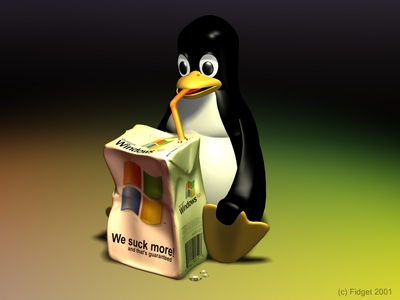
\includegraphics{tux.jpg}% a jpg image


foo bar baz foo bar baz

\begin{postscript}\rnode{foo}{foo} bar baz

foo bar baz foo bar \rnode{baz}{baz} foo bar baz
\ncarc[linecolor=red]{<->}{foo}{baz}\end{postscript}

foo bar baz

\begin{postscript}
\psframebox{%
\begin{pspicture}(-3,-2)(3,6.5)
\pstThreeDCoor[zMax=7]
\pstIIIDCylinder[RotY=30,fillstyle=solid,fillcolor=red!20,linecolor=black!60](0,0,0){2}{5}
\pstThreeDLine[linecolor=red]{->}(0,0,5)(0,0,7)
\pstThreeDLine[linecolor=red]{->}(-1,0,0)(4,0,0)
\pstThreeDLine[linecolor=red]{->}(0,-1,0)(0,4,0)
\end{pspicture}
}
\end{postscript}


\begin{postscript}
\begin{pspicture*}(-4,-2)(3,6.5)
\pstThreeDCoor[zMax=7]
\pstIIIDCylinder[RotY=30,fillstyle=solid,fillcolor=red!20,linecolor=black!60](0,0,0){2}{5}
\pstThreeDLine[linecolor=red]{->}(0,0,5)(0,0,7)
\pstThreeDLine[linecolor=red]{->}(-1,0,0)(4,0,0)
\pstThreeDLine[linecolor=red]{->}(0,-1,0)(0,4,0)
\end{pspicture*}
\end{postscript}


\end{document}
